\clearpage
\subsection{Terminal} % (fold)
\label{sub:terminal}

Once you have written some source code, you need to be able to compile it. This means, you need to run the \textbf{compiler}, and give it your source code files to compile. The best way to do this when you really want to learn about programming, is to run the compiler directly yourself. To do this you needed to use a \textbf{Terminal} program.

The Terminal is a program that gives you command line access to the computer. With command line access you can enter text commands to start programs. These programs can output details back to the Terminal for you to read, and interactive programs can also read input from you via this same Terminal.

\begin{figure}[h]
   \centering
   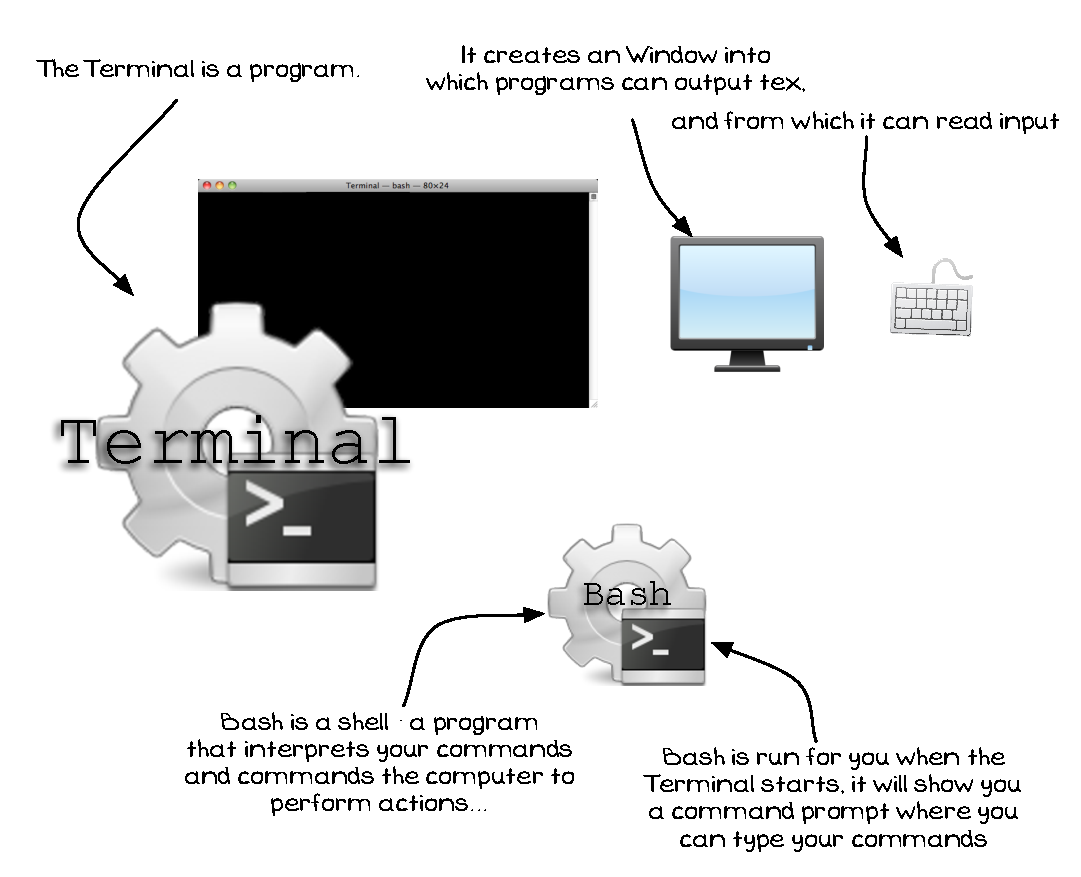
\includegraphics[width=0.8\textwidth]{./topics/programs-and-compilers/diagrams/Terminal} 
   \caption{The Terminal program gives you command line access to your computer}
   \label{fig:terminal}
\end{figure}

\mynote{
\begin{itemize}
  \item On Ubuntu \textbf{Linux} you can find the Terminal in the \emph{Accessories} folder within \emph{Applications}. See Figure \ref{fig:program-creation-ubuntu-terminal}.
  \item On \textbf{MacOS} you can find the Terminal in the \emph{Utilities} folder within \emph{Applications}. See Figure \ref{fig:program-creation-macos-terminal}.
  \item On \textbf{Windows} you will need to download and install \emph{MSys2}. The \emph{MSys2 Shell} is the equivalent of Terminal on the other operating systems. The details for how to install this are in the SplashKit installation guides.

  \item The Terminal is also be called the \textbf{console} or \textbf{command prompt}.
\end{itemize}
}

\clearpage
\subsubsection{The Shell} % (fold)
\label{ssub:the_shell}

The \textbf{Terminal} program itself just provides a text environment, allowing text input and output. Within this environment a \textbf{Shell} program is run to interpret your commands. This is an interactive program that will display a prompt to you, at which you enter your commands.

There are a number of different Shell programs, each of which has its own set of instructions. The Shell we are going to use in this book is called \textbf{Bash}. This shell program is available on Linux, Mac OS, and Windows. As a Unix shell it is native for Linux and Mac OS, and with Windows you can install \textbf{MSys2} to use these commands.

\begin{figure}[h]
   \centering
   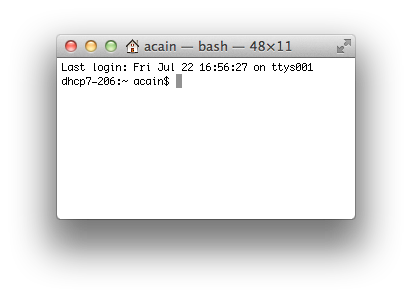
\includegraphics[width=0.6\textwidth]{./topics/programs-and-compilers/images/Bash} 
   \caption{The Terminal running Bash}
   \label{fig:bash}
\end{figure}

A shell program is very simple. It provides a text prompt at which you can enter commands. The Shell then reads the text you entered, and performs an action based on the text you entered. You can use the Shell to perform operations like copying and deleting files, and starting programs.

\mynote{
\begin{itemize}
  \item The name `Shell' came from idea that this was the outermost \emph{shell} of the computer, the interface between the user and the computer's internals.
  \item Bash stands for `\emph{Bourne-again shell}', as Bash is a replacement for the \emph{Bourne} shell.
  \item It will take some time to get used to using Bash, but the more you learn about it the more useful it will become.
\end{itemize}
}

% subsubsection the_shell (end)
\clearpage
\subsubsection{Using Bash} % (fold)
\label{ssub:bash}

To get started using Terminal you will need to know some Bash commands, see \tref{tbl:bash-commands}.

\begin{table}[h]
  \centering
  \begin{tabular}{|l|l|p{5cm}|}
    \hline
    \textbf{Action} & \textbf{Command} & \textbf{Description} \\
    \hline
    Change Directory & \texttt{cd} & Moves the shell to a different working directory. \\
    \hline
    Print Working Directory & \texttt{pwd} & Outputs the current working directory.\\
    \hline
    List Files & \texttt{ls} & Outputs a list of files.\\
    \hline
    Copy File(s) & \texttt{cp} & Copies files from one location to another.\\
    \hline
    Move File(s) & \texttt{mv} & Moves files from one location to another.\\
    \hline
    Delete File(s) & \texttt{rm} & Removes files from the computer. There is no recycle bin with this, so take care!\\
    \hline
    Create a Directory & \texttt{mkdir} & Makes a new directory. \\
    \hline
  \end{tabular}
  \caption{Some bash commands to get you started}
  \label{tbl:bash-commands}
\end{table}

To get started with Bash, you need to understand a little bit about the \textbf{file system}. Each operating system needs a way of storing its files, and there are going to be lots of files stored on a computer. This means that it would be cumbersome to try and keep these all in one place. Instead, the Operating System places files in \textbf{directories} (also known as \emph{Folders}). A directory can contain files, and other directories. 

When you are working in Bash, you will have a \textbf{working directory}. This is the directory where Bash will start searching for the files you are interacting with. To start working with the compiler you will need to be able to use the \textbf{change directory} command to move to the directory that contains your source code files.

With the \textbf{Change Directory} command you tell Bash which directory you want to move into, with the different parts of this path being separated by forward slashes (/). Example commands to move to your Documents directory are shown in \tref{tbl:dirs}, with screenshots for Linux in \fref{fig:linux-files}, Mac OS in \fref{fig:mac-files}, and Windows in \fref{fig:win-files}.

\begin{table}[h]
  \centering
  \begin{tabular}{|l|l|}
  \hline
  \textbf{Operating System} & \textbf{CD Command}  \\
  \hline
  \emph{Linux} & \texttt{cd /home/\emph{uname}/Documents} \\
  or & \texttt{cd $\sim$/Documents} \\
  \hline
  \emph{Mac OS} & \texttt{cd /Users/\emph{uname}/Documents} \\
  or & \texttt{cd $\sim$/Documents} \\
  \hline
  \emph{Windows} & \texttt{cd /c/Users/\emph{uname}/Documents} \\
  \hline
\end{tabular}
  \caption{CD command to move into your documents directory on various Operating Systems. In these examples \texttt{\emph{uname}} should be replaced by your user name. The examples in \fref{fig:linux-files}, \fref{fig:mac-files}, and \fref{fig:win-files} are for the user \texttt{acain}.}
  \label{tbl:dirs}
\end{table}

\mynote{
\begin{itemize}
  \item You can find many resources on using Bash on the web, a fairly extensive overview of these commands can be found at \url{https://dev.to/awwsmm/101-bash-commands-and-tips-for-beginners-to-experts-30je}.
  \item After you run the \texttt{cd} command, you can check which directory you are in using the \textbf{pwd} command. To do this just type \texttt{pwd} and press enter.
  \item Once you get used to the \texttt{cd} command you can start exploring the other commands.
\end{itemize}
}

\begin{figure}[p]
   \centering
   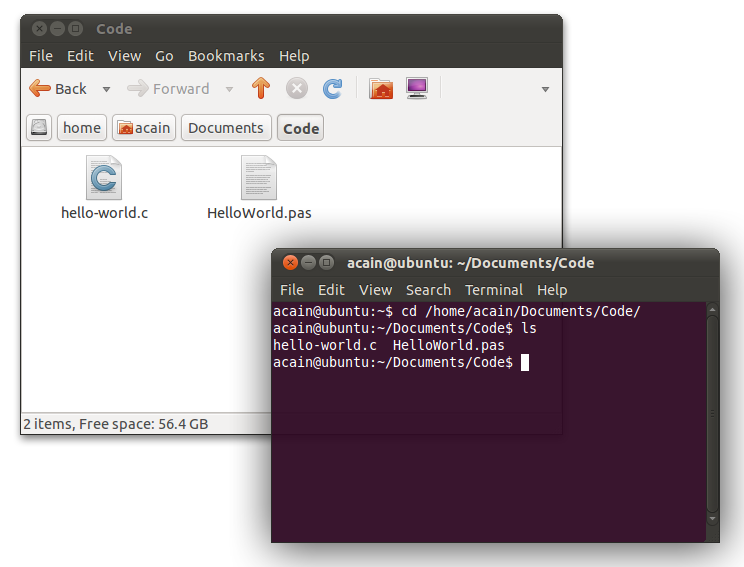
\includegraphics[width=0.9\textwidth]{./topics/programs-and-compilers/images/LinuxFiles} 
   \caption{Changing directories in Linux (Ubuntu)}
   \label{fig:linux-files}
\end{figure}

\begin{figure}[p]
   \centering
   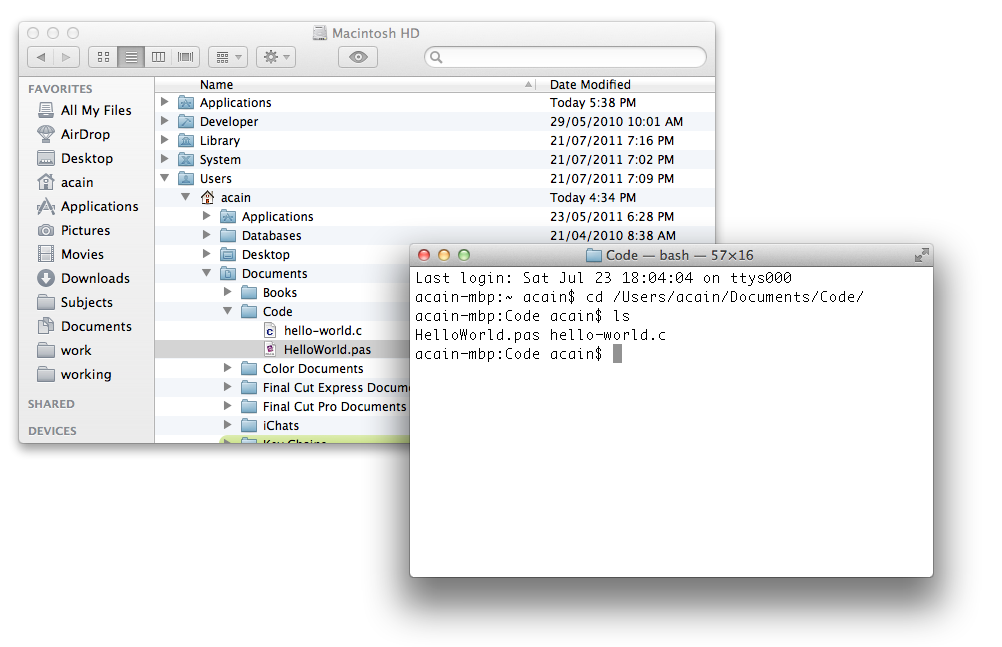
\includegraphics[width=0.9\textwidth]{./topics/programs-and-compilers/images/MacFiles} 
   \caption{Changing directories in MacOS}
   \label{fig:mac-files}
\end{figure}


\begin{figure}[p]
   \centering
   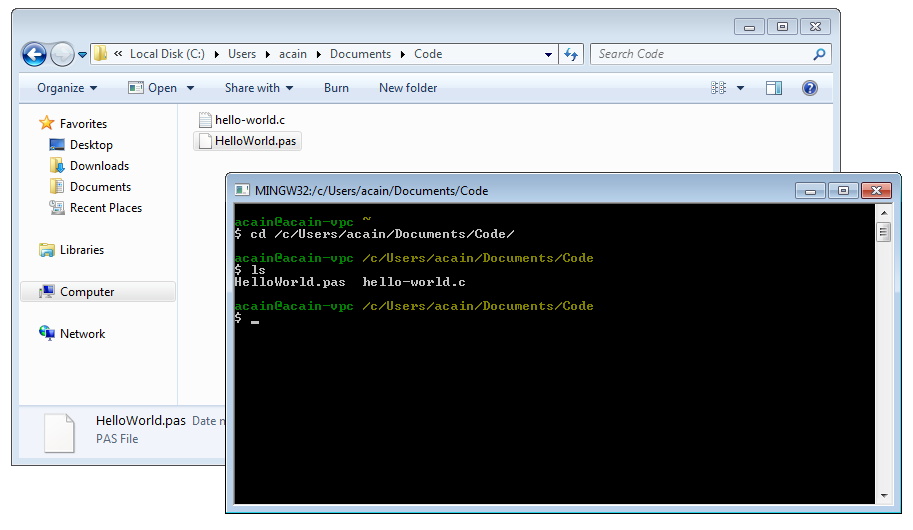
\includegraphics[width=\textwidth]{./topics/programs-and-compilers/images/WindowsFiles} 
   \caption{Changing directories in Windows}
   \label{fig:win-files}
\end{figure}



% subsubsection bash (end)

% subsection terminal (end)